% Chapter Template

\chapter{Basics Related Roncepts} % Main chapter title

\label{c3} % Change X to a consecutive number; for referencing this chapter elsewhere, use \ref{ChapterX}

%----------------------------------------------------------------------------------------
%	SECTION 1
%----------------------------------------------------------------------------------------
\section{Deep learning models}
\subsection{Convolutional Neural Network (CNN)}
A CNN is an essential neural network utilised extensively for analysing time series and processing signals. Unlike standard fully connected neural networks,  which process input as vectors,  1D CNNs extract local features using convolution operations using a sliding window technique. They're made to operate with one-dimensional signals like audio or time series sensor readings. In \Cref{CNN} \cite{chaerun2021comparative} 1D CNN,  multiple filters are employed to extract various features from the input signal. These filters slide over the input,  capturing local patterns and representations. The convolutional layer output is then downsampled using pooling layers,  reducing the data dimension and preventing overfitting. The network may also include fully connected layers that perform tasks like classification or regression using the retrieved features.
\par The simplicity of the 1D CNN \cite{kiranyaz20211d} architecture lies in its effectiveness in extracting features from one-dimensional signals. The sliding window approach allows the network to focus on local details and extract relevant information effectively. Furthermore,  the convolutional process reduces the number of parameters,  resulting in a more computationally efficient network. Pooling layers help in generalisation by decreasing output complexity,  resulting in higher performance on previously unknown data. 1D CNNs are versatile and practical in various domains since they can examine historical data and extract relevant characteristics. They've shown to be incredibly effective in applications such as speech recognition \cite{rusnac2022cnn, wang2019end},  audio categorisation \cite{ashraf2022role, hu2020device},  and sensor data processing \cite{kattenborn2021review, sun2019classification}. Overall,  1D CNNs are potent tools for collecting features from one-dimensional data,  providing essential insights,  and paving the way for signal processing and time series analysis advances.

\begin{figure*}[h!]
  \centering
    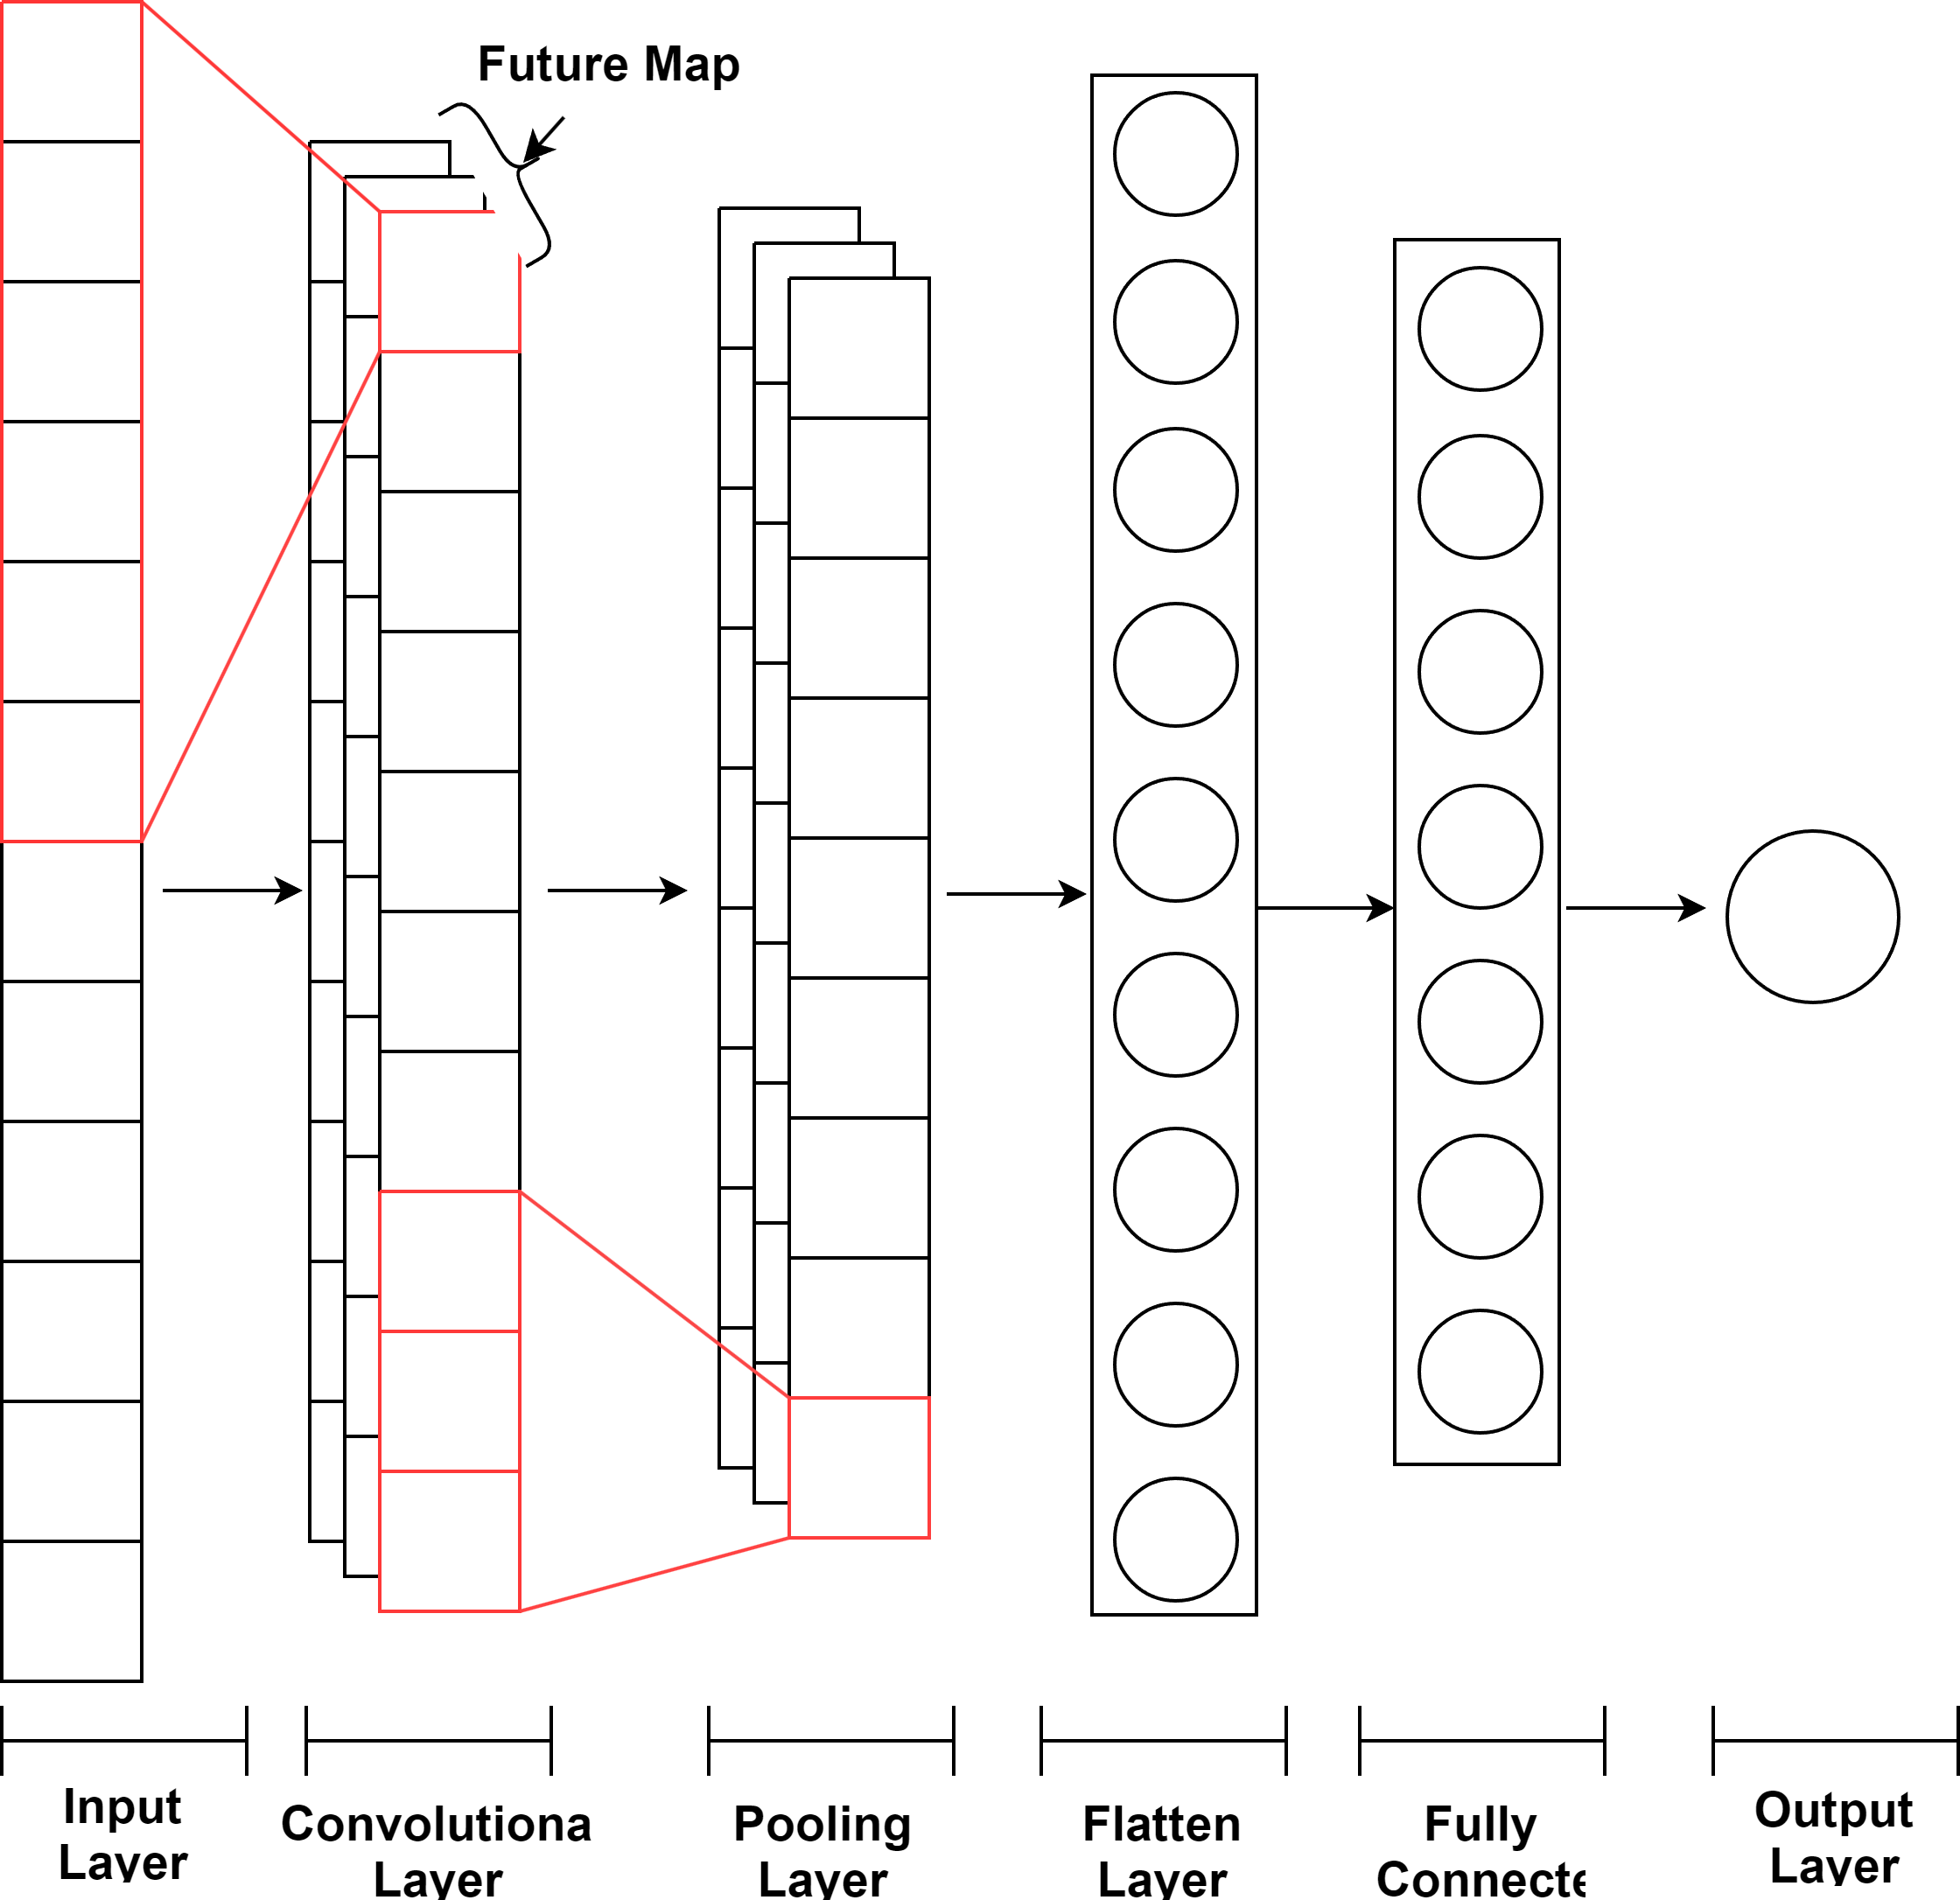
\includegraphics[scale=.8]{cnn}
    \caption{Traditional architecture of $1D-CNN$}\label{CNN}
\end{figure*}

1D CNN uses a set of learnable filters (or kernels) of length k to conduct the convolution operation. This operation involves computing the dot product between the filter and a k-length window sliding over the input sequence x with length L. Then a new sequence of feature maps is generated as an outcome.

\par Denoting the set of filters as $F$ and the output feature map at position $i$ as $h_i$,  we can express the output feature map $h$ as follows: 
\begin{equation}\label{equ: cnn}
        h_i = \sigma \left(\sum_{j=1}^{k}F_{j}.x_{i+j-1}+b \right)
\end{equation}
Where $F_j$ represents the $j^{th}$ filter in the set of filters $F$,  $x_{i+j-1}$ is the value of the input sequence $x$ at position $(i+j-1)$,  $\sigma$ is the activation function (such as ReLU or sigmoid),  and $b$ is the bias term.

\subsection{Gated Recurrent Unit (GRU)}
The GRU is a specialised recurrent neural network architecture designed for managing sequential data input  \cite{chung2014empirical}, and the unique proposal was put forth as a substitute for the well-liked LSTM network. These gating mechanisms selectively update the hidden state,  allowing GRU to capture dependencies in sequential data effectively. GRU has found use in an array of areas,  including speech recognition \cite{shewalkar2019performance, yuan2018auxiliary},  natural language processing \cite{cascianelli2018full, wang2020feature},  and picture recognition \cite{subramanian2022integrated},  due to its gating mechanisms and ability to handle sequential dependencies. Its capabilities make it a powerful tool for modelling and understanding sequential data,  providing valuable insights and improved performance in numerous tasks. GRU network based on gates and states are shown in \Cref{up Gru} to \Cref{hid gru}: \\
Update Gate :
\begin{equation} \label{up Gru}
  z_t= \sigma(W_{z}\cdot \left[ h_{t-1}, x_t \right]+b_z )
\end{equation}
Reset Gate : 
\begin{equation}\label{r gru}
 r_t=\sigma (W_{r}\cdot \left[ h_{t-1}, x_t \right]+b_r )
\end{equation}
Candidate activation :
\begin{equation} \label{can gru}
    \tilde{h_t}=tanh(W_h \cdot \left[ r_t \odot h_{t-1}, x_t \right]+b_h)
\end{equation}
Hidden State :  
\begin{equation} \label{hid gru}
  h_t=(1-z_t) \odot h_{t-1}+z_t \odot \tilde{h_t}
\end{equation}



where,  time step t,  the hidden state is represented by $ h_t $,  the input is represented by $ x_t $,  and the update and reset gates are
represented by $ x_t $ and $ r_t$ respectively. The refresh entryway directs the amount of the past covered state to keep for the present time step,  while the reset entryway controls the amount of the past covered state to overlook. The candidate activation $\tilde{h_t}$ represents new information that could be added to the hidden state. The sigmoid activation function $ \sigma $ and element-wise multiplication represented by $\odot$ are used.Weight matrices $ W_z $,  $ W_r $,  $ W_h $ and bias vectors $ b_z $,  $ b_r $,  $ b_h $ are also utilized. The GRU's update and reset gates allow it to learn when to update the hidden state and what information to forget,  making it particularly useful for modelling sequential data with long-range dependencies.
\subsection{Recurrent Neural Network (RNN)}
RNN is an ANN that utilises the outcome of the preceding measure to contribute to the present step. Forecasting the succeeding phrase in a statement is not a strong suit of RNNs because their Memory State,  also recognised as the hidden layer,  does not preserve any data about preceding words. It stores the previous input given to the network,  which goes a long way in ensuring accurate predictions. The RNN technique employs identical parameters for every input,  leading to it executing the same function on every hidden layer to obtain the results. Unlike other neural networks, it significantly reduces the complexity of parameters,  making it a popular choice among researchers and developers. The elegance of RNN rests in its capacity to recall prior inputs,  rendering it a valuable instrument in creating predictions that demand context. Ordinarily,  profound learning has been exhibited to be a game-changer in AI and ML,  and it will undoubtedly persist in being an essential instrument in the coming years.

Recurrent Neural Network (RNN) model are input \& output to hidden state can be written as \Cref{equ: ih rnn} \& \Cref{equ: h rnn} respectiveely: \\
Input to Hidden State:
  \begin{equation} \label{equ: ih rnn}
    h_t= \psi (W_{hx} \cdot x_t + W_{hh} \cdot h_{t-1} +b_h)
  \end{equation}
  Hidden State to Output: 
  \begin{equation} \label{equ: h rnn}
     y_t=W_{yh}\cdot h_t+b_y
  \end{equation}
where $h_t $ is the hidden state at time step $t$,  $x_t$ is input at $t$ step of time,  $y_t$ is output at t step of time,  $W_{hx} $ is a weight matrix that links the input to the concealed state,  $W_{hh}$ is the weighted matrix that connects the state that is hidden at time step $t-1$ with the hidden value step t,  $W_{yh}$ is a weighted matrix that links the state that is hidden to the output,  $b_h$ and $b_y$ are biassed terms for both the state that is hidden and the output and $\psi (\cdot)$ is a function of activation applied to the concealed state element by element.


\subsection{Long-Short-Term Memory (LSTM)}
LSTMs are a specialised type of RNN designed to handle sequential data. They excel at learning long-term dependencies,  making them suitable for language translation,  speech recognition,  and time series forecasting. Utilising the memory cell and three gates facilitates the capability of LSTMs to learn intricate patterns in data by selectively retaining and discarding information. Deep LSTM networks,  achieved by stacking LSTMs,  are beneficial for tasks like speech recognition \cite{soltau2016neural, jo2020approximate} and natural language processing \cite{wang2015learning, nammous2019natural}. Hochreiter and Schmidhuber  \cite{hochreiter1997long} developed LSTMs to overcome the long-term dependency issue in traditional RNNs. LSTMs are widely used in processing \cite{sahin2018nonuniformly},  prediction \cite{gers2000learning},  and classification \cite{zhou2015c, karim2017lstm} of temporal data,  and when combined with CNNs,  they efficiently analyse images \cite{li2019cnn, rajendran2020land, islam2020combined} and videos \cite{ullah2017action, li2020classifying, gao2017video, bin2018describing} by extracting spatial and temporal features. LSTMs are an effective instrument for analysing sequential data and can be incorporated with other neural network structures to accomplish more complex objectives.
The LSTM architecture-related gates and states are shown in \Cref{lstm i} to \Cref{lstm h}.\\
Input Gate : 
  \begin{equation} \label{lstm i}
     i_t=\sigma (W_{xi}\cdot x_t+W_{hi}\cdot h_{t-1}+b_i)
  \end{equation}
  Forget Gate : 
  \begin{equation}\label{lstm f}
    f_t= \sigma(W_{xf}\cdot x_t +W_{hf}\cdot h_{t-1}+b_f)
  \end{equation}
  Candidate Hidden State :
  \begin{equation}\label{lstm c}
       g_t=than(W_{xg}\cdot x_t+W_{hg}\cdot h_{t-1} +b_g)
  \end{equation}
  Cell State :
  \begin{equation}\label{lstm ce}
  C_t=f_t \odot C_{t-1}+i_t \odot g_t
  \end{equation}
  Output Gate : 
  \begin{equation}\label{lstm o}
    o_\sigma(W_{xo}\cdot x_t +W_{ho}\cdot h_{t-1}+b_o)
  \end{equation}
  Hidden State :
  \begin{equation} \label{lstm h}
      h_t=o_t \odot tanh(C_t)
  \end{equation}
whare,  $h_t$ at a time step,  is the concealed condition (also known as a hidden representation),  $x_t$  is the time step input,  $C_t$  is the condition of the cell at time step $t$,  serving as the LSTM's long-term memory,  $\sigma$ Its sigmoid activation function,  The tangent hyperbolic activation function is denoted by tanh,  $\odot$ represents element-by-element multiplication,  $W_{xi}$,  $W_{hi}$,  $W_{xj}$,  $W_{hf}$,  $W_{xg}$,  $W_{hg}$,  $W_{xo}$,  $W_{ho}$ are the matrices of that will be taught throughout training and $b_i$,  $b_f$,  $b_g$,  $b_o$ are slanted terms.


\subsection{Bi-directional Long Short Term Memory (BiLSTM)}
BiLSTM is a type of human stupidity designed to process sequential data in neither forward nor backward directions. The plan uses dual LSTM layers for forward and backward processing concurrently,  enabling it to grasp the context from previous and upcoming time steps. Therefore,  the network cannot identify any relationships in either direction,  making it a disadvantage for speech recognition and language translation tasks. By providing a broader perspective of the input sequence,  BiLSTMs can improve the performance in tasks requiring contextual understanding. These forms are remarkable for long-term dependencies and are commonly utilised in profound learning projects.

\begin{figure*}[h!]
  \centering
  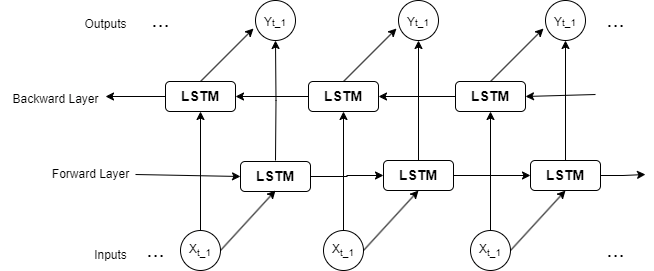
\includegraphics[scale=0.8]{Bilstm}
  \caption{Architecture of BiLSTM \cite{article}} \label{Bilstm}
\end{figure*}



BiLSTM network architecture gates and states are shown below from \Cref{bi i} to \Cref{bi h}.\\
\begin{itemize}
  \item  Forward LSTM: \\
  Input Gate : 
    \begin{equation} \label{bi i}
    i_t^f = \sigma(W_{xi}^f \cdot x_t + W_{hi}^f \cdot h_{t-1}^f + W_{ci}^f \cdot c_{t-1}^f + b_i^f)
    \end{equation}
    Forget Gate : 
    \begin{equation}
      f_t^f = \sigma(W_{xf}^f \cdot x_t + W_{hf}^f \cdot h_{t-1}^f + W_{cf}^f \cdot c_{t-1}^f + b_f^f) 
    \end{equation}
    Candidate Hidden State :
    \begin{equation}
        g_t^f = \text{tanh}(W_{xg}^f \cdot x_t + W_{hg}^f \cdot h_{t-1}^f + b_g^f)
    \end{equation}
    Cell State : 
    \begin{equation}
      c_t^f = f_t^f \odot c_{t-1}^f + i_t^f \odot g_t^f
    \end{equation}
    Output Gate : 
    \begin{equation}
   o_t^f = \sigma(W_{xo}^f \cdot x_t + W_{ho}^f \cdot h_{t-1}^f + W_{co}^f \cdot c_t^f + b_o^f)
    \end{equation}
    Hidden State : 
    \begin{equation} \label{bi h}
    h_t^f = o_t^f \odot \text{tanh}(c_t^f) 
    \end{equation}

  \item Backward LSTM: 
  The formulas for the rear LSTM are similar to those of the forward LSTM but with different weights and biases. The superscript "b" is used to denote the backward direction (e.g.,  \(W_{xi}^b\) is the weight matrix for the input gate in the backward LSTM). The BiLSTM combines the hidden forward and backwards states to form the final output. The output \(y_t\) at time step \(t\) is typically computed using a combination of both forward and backwards hidden states. The approach for combining the two directions (e.g.,  concatenation,  addition,  etc.) depends on the specific task and model architecture.
\end{itemize}

\section{ Performance Measures}
\subsection{Root Mean Square Error (RMSE) }
The RMSE is hardly ever utilised as a standard for assessing the precision of a regression model. The computation of the root mean square of discrepancies between projected and factual figures can facilitate identifying the divergence between them while keeping the units of measurement consistent with the data. This provides valuable insight into the model's effectiveness. A lower RMSE digit suggests superior model performance,  while an increased RMSE value indicates substandard model performance. The RMSE \Cref{rmsee} uses metrics for regression models by effectively evaluating the model's accuracy,  as it quantifies the discrepancy between projected and actual values in the same unit as the data. By analysing the RMSE score,  experts can evaluate the model's efficacy and implement necessary tweaks to enhance its precision. As a final point,  the RMSE is a crucial statistic for evaluating the accuracy of regression models,  and its usage is essential in industries that heavily depend on data science,  finance,  and engineering.

\begin{equation} \label{rmsee}
  RMSE=\sqrt{\frac{\sum_{i=1}^{n}(y_{i}-\hat{y_{i}})^2}{n}}
\end{equation}
where $n$ represents the number of times that the summation iteration occurs,  \begin{math} y_{i} \end{math} denotes the actual value,  and \begin{math}\hat{y_{i}}\end{math} represents the forecast value.

\subsubsection{ Mean Absolute Percentage Error (MAPE)}
  A popular metric for judging the efficiency of regression models is MAPE. It measures the percentage of variance between predicted and actual results and averages these discrepancies. MAPE can be computed by finding the average of the absolute percentage errors between the expected and actual values,  such as \Cref{mapee}.
\begin{equation} \label{mapee}
  MAPE=\frac{1}{n}\sum_{i=1}^{n} \left | \frac{y_{i}-\hat{y_{i}}}{y_{i}} \right |
\end{equation}
where $n$ represents the number of times that the summation iteration occurs,  \begin{math} y_{i} \end{math} denotes the Actual value,  and \begin{math}\hat{y_{i}}\end{math} represents the forecast value.

MAPE determines the average percentage discrepancy between the projected and observed values. In business and finance,  it is a common practice to assess the precision of forecasts or predictions using this technique. Industries utilise MAPE to compute the mean percentage deviation between anticipated and actual values,  where a lower value suggests better model performance and a higher value suggests poorer performance. However,  MAPE can cause division by zero errors or huge percentage errors when the actual numbers are close to zero.



